\documentclass[a4paper]{report}
\usepackage[utf8]{inputenc}
\usepackage[T1]{fontenc}
\usepackage[x11names, rgb]{xcolor}
\usepackage{a4wide}
\usepackage{lscape}
\usepackage{hyperref}
\usepackage{longtable}
\usepackage{syntax}
\hypersetup{pdftitle={Processing an Angolan Newspaper},
pdfauthor={Pedro Mendes},
colorlinks=true,
urlcolor=blue,
linkcolor=black}
\usepackage{subcaption}
\usepackage[cache=false]{minted}
\usepackage{listings}
\usepackage{booktabs}
\usepackage{multirow}
\usepackage{appendix}
\usepackage{tikz}
\usepackage{amsmath}
\usetikzlibrary{snakes,arrows,shapes}

\begin{document}

\title{Informatics Dictionary}
\author{Pedro Mendes (a79003)}
\date{\today}

\begin{center}
    \begin{minipage}{0.75\linewidth}
        \centering
        
\includegraphics[width=0.4\textwidth]{eng.jpeg}\par\vspace{1cm}
        \vspace{1.5cm}
        \href{https://www.uminho.pt/PT}
        {\color{black}{\scshape\LARGE Universidade do Minho}} \par
        \vspace{1cm}
        \href{https://www.di.uminho.pt/}
        {\color{black}{\scshape\Large Departamento de Informática}} \par
        \vspace{1.5cm}
        \maketitle
    \end{minipage}
\end{center}

\begin{abstract}
    \begin{center}
    \end{center}
\end{abstract}

\tableofcontents

\pagebreak

\chapter{Introduction}

This project aims to create a simple and intuitive language to describe a
dictionary and later annotate texts with.

First we'll analyse the problem, see what needs to be implemented and what
challenges need to be overcome to implement said features.

Next we'll look at the solutions to the proposed problems, dedicating a
section to the solution of each problem.
% TODO: FINISH THIS

\chapter{Problem}

The problem this program intends to solve is the following, the informatics
department wants to create a dictionary of commonly used words, associating
with each of them a \textit{meaning}, the \textit{English name} and a list of
\textit{synonyms}. This dictionary is read in conjunction with texts (that may
or may not contain a title) and annotates them with footnotes explaining the
words that are defined in the dictionary.

To solve this problem, a DSL\footnote{Domain Specific Language} needs to be
defined where the dictionary can be stored as well as texts to annotate. It's
also important that the language is user friendly as it is intended to be
human readable and writeable.

\chapter{Solution}\label{cha:solution}

\section{Definition of the SATI language}

Similarly to how an imperative
program is split in two, declarations and instructions, this language is split
between dictionary (\textit{Dicl}) and texts (\textit{Texts}), separated by one or more `\verb!\%!'.

\lstinputlisting[firstline=10,lastline=12,basicstyle=\footnotesize\ttfamily]
{../src/sati.y}

\subsection{Dictionary}

The dictionary is a collection of words and each word is composed of 4 parts.

\begin{grammar}
    <dicl> $\to$ <word>
    \alt{} <dicl> <word>
\end{grammar}

The word to find in the dictionary \textit{WD}, it's meaning \textit{Meaning}
the \textit{English Name} and finally either a list of synonyms or a single
synonym.

The list of synonyms contains synonyms separated by \verb!','! and the last one
on the list may or may not be followed by a comma.

\begin{grammar}
    <word> $\to$ <wd> `:' <meaning> `|' <englishName> `|' `[' <synonyms> `]' `;'
    \alt{} <meaning> `|' <englishName> `|' <synonym> `;'

    <synonyms> $\to$ <synonym> `,'
    \alt{} <synonyms> <synonym> `,'
    \alt{} <synonyms> <synonym>

    <wd> $\to$ <ID>

    <meaning> $\to$ <ID>

    <englishName> $\to$ <ID>

    <synonym> $\to$ <ID>
\end{grammar}

As an example, a dictionary can be written like this:

\begin{verbatim}
Encapsulamento : Um mecanismo da linguagem para
                 restringir o acesso aos componentes
                 de um objecto.
               | Encapsulation
               | Modularidade
               ;

Imutabilidade : Uma propriedade de informação que
                implica que esta não pode ser alterada.
              | Imutability
              | [ Constante, Inalteravel, ]
              ;
\end{verbatim}

\inputminted[firstline=17,lastline=36]{C}{../src/sati.y}

\section{Texts}

The texts section is composed of texts that may or may not have a title, the
title is used to name the \LaTeX{} chapter, if no title is given then
\textit{Untitled X} will be used where \textit{X} is the number of untitled
texts parsed so far.

The texts are surrounded by double quotes \verb!"! and their title is text
preceding the text. The language specification for presenting the texts is the
following:

\begin{grammar}
<texts> $\to$ `\"' <text> `\"'
      \alt{} <texts> `\"' <text> `\"'
      \alt{} <texts> <title> `\"' <text> `\"'
      \alt{} <title> `\"' <text> `\"'

<text> $\to$ <TEXT>

<title> $\to$ <TEXT>
\end{grammar}

And a sample text section could be:

\begin{verbatim}
POO "O encapsulamento permite uma maior modularidade e organização do código."
"Em programação é muito importante o single responsability principle."
\end{verbatim}

\begin{figure}[H]
    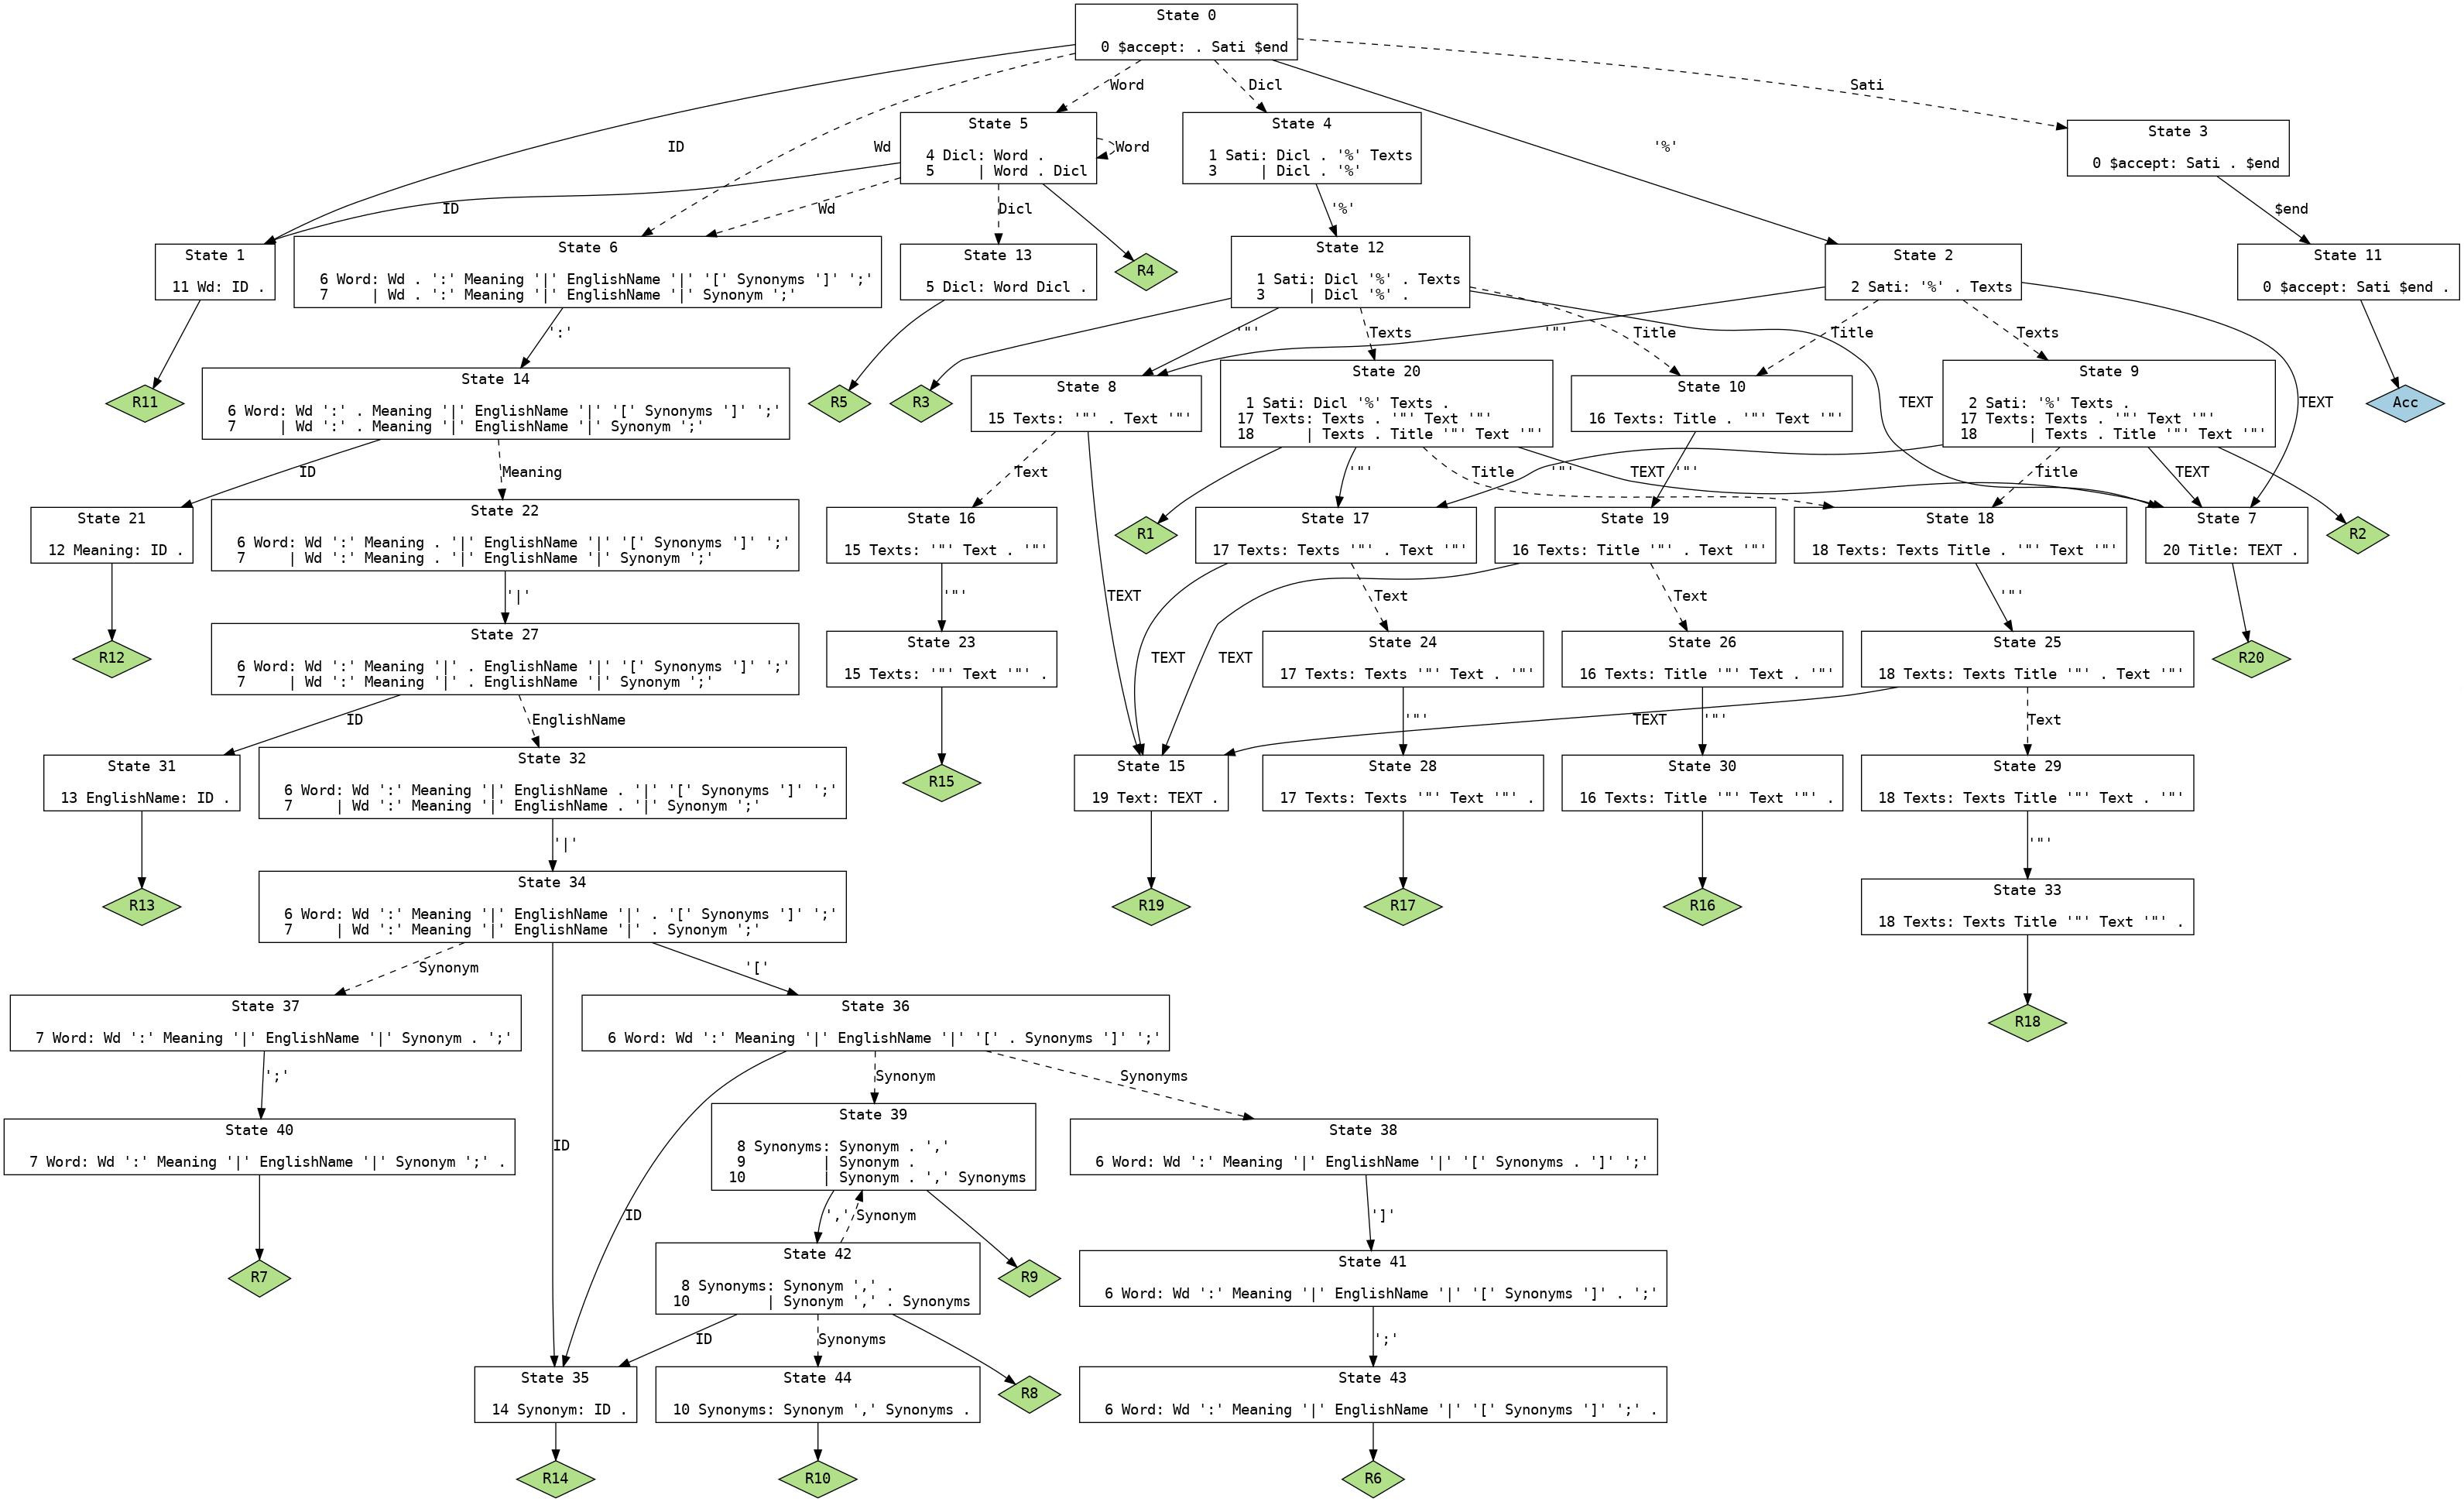
\includegraphics[width=\textwidth]{./sati.jpg}
    \caption{The Parser's Automata generated by \textit{yacc}}
\end{figure}

And the full SATI file can be something like this.

\begin{verbatim}
Encapsulamento : Um mecanismo da linguagem para
                 restringir o acesso aos componentes
                 de um objecto.
               | Encapsulation
               | Modularidade
               ;

Imutabilidade : Uma propriedade de informação que
                implica que esta não pode ser alterada.
              | Imutability
              | [ Constante, Inalteravel, ]
              ;
%%
POO "O encapsulamento permite uma maior modularidade e organização do código."
"Em programação é muito importante o single responsability principle."
\end{verbatim}

\section{Architecture}

\section{Usability/Flags}

\chapter{Conclusion}

\appendix

\chapter{GIC}

\lstinputlisting[firstline=10,lastline=48,basicstyle=\footnotesize\ttfamily]
{../src/sati.y}

\chapter{Flex}

\lstinputlisting[firstline=11,lastline=15,basicstyle=\footnotesize\ttfamily]
{../src/sati.l}

\end{document}

